\documentclass[float=false, crop=true]{standalone}

\usepackage{tikz}
\usepackage{graphicx}

\usetikzlibrary{automata, positioning, arrows.meta}                             % Tikz macros

\begin{document}
\resizebox{0.45\columnwidth}{!}{%
  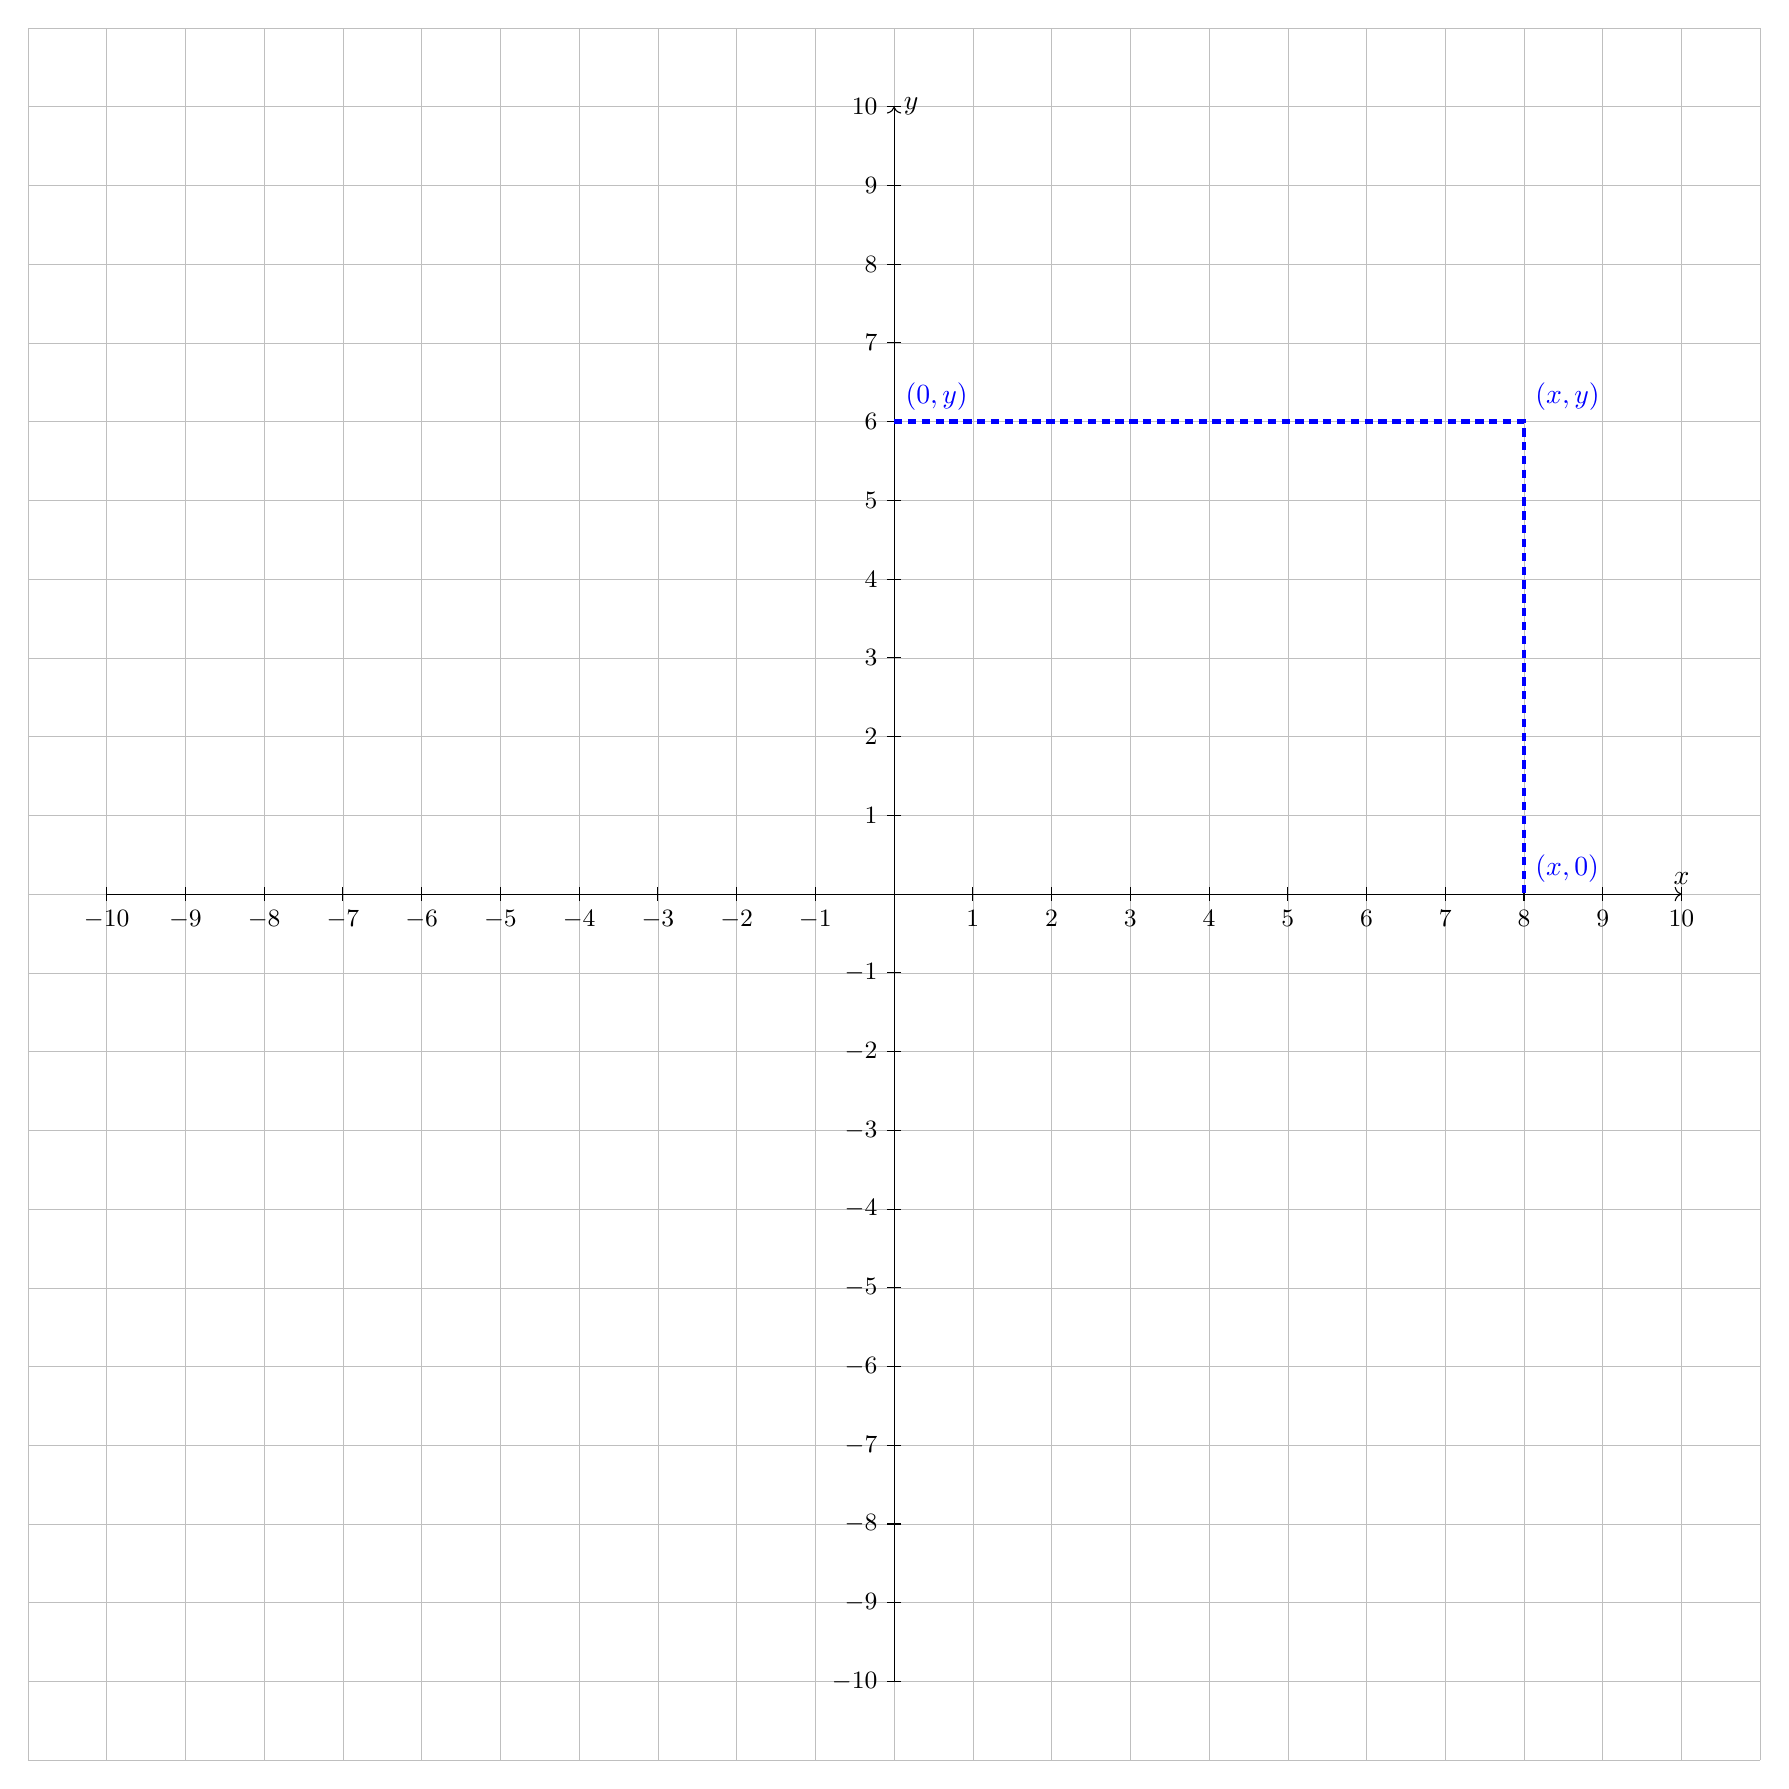
\begin{tikzpicture}
    \path [draw, help lines, opacity=.5]  (-11,-11) grid (11,11);
    \foreach \i in {1,...,10} \draw (\i,2.5pt) -- +(0,-5pt) node [anchor=north, font=\small] {$\i$} (-\i,2.5pt) -- +(0,-5pt) node [anchor=north, font=\small] {$-\i$} (2.5pt,\i) -- +(-5pt,0) node [anchor=east, font=\small] {$\i$} (2.5pt,-\i) -- +(-5pt,0) node [anchor=east, font=\small] {$-\i$};
    \draw [->] (-10,0) -- (10,0) node [anchor=south] {$x$};
    \draw [->] (0,-10) -- (0,10) node [anchor=west] {$y$};
    \path [draw=blue, ultra thick, text=blue, densely dashed] (0,6) node [anchor=south west] {$(0,y)$} -| (8,0) node [anchor=south west] {$(x,0)$} node [anchor=south west, midway] {$(x,y)$};
  \end{tikzpicture}%
}

\end{document}
